\chapter{Literature Review}\label{C:lit}

The analysis of complex time series has long relied on both time-domain and frequency-domain techniques. 
However, traditional methods often fall short in capturing nonlinear dynamics or are limited by strict assumptions such as stationarity and Gaussianity. 

The ordinal symbolic approach introduced by Bandt and Pompe in 2002 marked a significant theoretical advance by enabling robust, model-free characterization of time series. 
Their approach, rooted in information theory, involves converting segments of time series data into symbols based on the ordinal (rank) relationships among the data points.
These symbols are called "ordinal patterns." After computing all the symbols, their relative frequencies are used to estimate the probability distribution of ordinal patterns.

From this distribution estimate, two key descriptors entropy and complexity are calculated to characterize the time series: the scaled Shannon entropy, now widely known as permutation entropy, and the statistical complexity.

López-Ruiz et al.~\cite{lopez1995statistical} to capture the structure of a system. By plotting permutation entropy against statistical complexity, Rosso et al.~\cite{Rosso2007} use the entropy-complexity plane as a powerful diagnostic tool to distinguish between different dynamical regimes, such as chaos, noise, and periodicity.

%%% 
%%% ACF We need the statistical complexity here
This chapter is divided into three main sections. The first section discusses the emergence of the entropy-complexity plane. This topic is presented as a central theme because it reflects the foundation of our main research focus and illustrates how it has evolved over time into the current approach to time series analysis based on the concept of ordinal patterns.
The second section analyzes the bibliometrix results derived from references that cite the Bandt and Pompe methodology. The third section presents a literature review based on the insights gained through the bibliometrix analysis. Bibliometrix is primarily used to quantify scientific production and assess its quality and impact. It is a widely adopted quantitative approach in systematic literature reviews, useful for mapping the intellectual structure, identifying research trends, and highlighting key contributions within a specific field. Additionally, it helps visualize and analyze the intellectual, conceptual, and social structures of research. The main objective of bibliometrix analysis is to describe how specific disciplines or scientific domains are organized and how they evolve over time.

Following this analysis, we focus our literature review on the most relevant aspects identified in relation to our research topic. By examining citation patterns and bibliographic data from the Scopus database, this review identifies the theoretical foundations and practical applications of the Bandt–Pompe methodology. The decision to use bibliometrix analysis was motivated by its ability to provide an objective assessment of influential publications, collaboration networks, and emerging research themes, thereby enhancing both the transparency and reproducibility of the review process.
%Recent developments and challenges in this area are also highlighted, including insights from comprehensive reviews by Amigó et al.\cite{amigo2023ordinal} and Leyva et al.\cite{Leyva2022}.


\section{The Onset of the Entropy-Complexity Plane}

%%% ACF Anticipate briefly what this is about 

%Bandt and Pompe~\cite{PhysRevLett.88.174102} introduced in 2002 a novel approach to time series analysis by focusing on the ordinal relationships between data points rather than their actual values. 
%This method involves mapping a time series into a sequence of symbols representing the relative ordering of values within embedding vectors. 
%The authors computed the scaled Shannon entropy (the permutation entropy) of the frequency distribution of these patterns, and used it as a measure of the signal complexity.
%Since the symbols are invariant under monotonic increasing transformations and robust to observational noise and errors, 
%%% ACF Think about "noise" and "error"; see if you find better words for them
%so is any feature derived from them.
%This approach requires minimal assumptions about the data, it is computationally efficient, and effective for short time series, making it suitable for a wide range of applications~\cite{Zanin2012}.


Bandt and Pompe introduced a method for symbolizing time series in 2002, based on two key parameters: embedding dimension and time delay. In their approach, a time series is converted into a sequence of symbols, which are then used to estimate a probability distribution function, often represented as a histogram. From this probability distribution, they calculate permutation entropy.

However, permutation entropy alone is not sufficient to fully analyze time series data. To address this, Martin et. al.~
\cite{Martin2003}. introduced the the concept of disequilibrium as an essential ingredient of a family of statistical complexity measure in 2003. They found that the use of Euclidean distances for probability space become quite relevant to this endeavor, building on the concept of complexity previously proposed by López-Ruiz et al.~\cite{lopez1995statistical} in 1995. López-Ruiz defined complexity using Shannon entropy and the Euclidean distance between the observed probability distribution and the uniform distribution.

Recognizing limitations in this approach, Lamberti et al.~\cite{lamberti2004intensive} further examined the properties of complexity and refined the measure by incorporating the Jensen–Shannon divergence instead of the Euclidean distance. Further, Martin et.al.~\cite{Martin2006} discussed bounded values adopted by the generalized statistical complexity measures. Finally, Rosso et.al.~\cite{Rosso2007} then defined complexity separately and combined it with permutation entropy to form the entropy-complexity plane, providing a more robust framework for analyzing time series data.
%The Shannon entropy is employed to quantify the unpredictability or complexity of the symbolic sequence. 
%The resulting permutation entropy has several attractive properties: it is computationally efficient, non-parametric, ~\cite{ Zanin2012}. 
%%% ACF A statistical measure of complexity discussed how C must behave, and the authors proposed a (not so good) way of computing it
%%% ACF {EEG} analysis using wavelet-based information tools proposes the Jensen-Shannon distance, that leads to the statistical complexity as we use it.
%A further theoretical development by López-Ruiz et al.~\cite{lopez1995statistical} extended method by introducing the statistical complexity, which measures both the system's randomness and structure. 
%%% ACF They couldn't have extended a method that was proposed ahead in time
%%% ACF Revise the following sentence
%%% ACF There is a previous article
%Later, Rosso et al.~\cite{Rosso2007} extended and applied statistical complexity in the entropy-complexity plane framework,
%Plotting the permutation entropy against the statistical complexity yields the entropy-complexity plane, a diagnostic tool for classifying different dynamical regimes.

\section{The Bibliometrix Analysis: data collection, tools and background}
Bibliometric analysis provides a quantitative approach to reviewing and mapping the intellectual structure of a research field. By systematically analyzing the citation patterns, author collaborations, and keyword co-occurrences within the literature, it allows for the identification of key themes, research trends, and emerging topics. In this study, bibliometric analysis was conducted using the Bibliometrix package in R and its user-friendly web interface Biblioshiny, focusing on literature related to ordinal patterns, permutation entropy, and complexity measures in time series analysis.

Scopus-indexed references that cited the seminal work by Bandt and Pompe were collected on the 9th of June 2025. Based on these reference files, we analyzed a dataset consisting of 4125 reference files spanning the years 1993 to 2025. Keywords used for data extraction included Bandt and Pompe research, ordinal patterns, permutation entropy, and time series clustering. The aim of this bibliometric analysis was to identify and classify the literature according to application domains and theoretical developments related to ordinal patterns in time series analysis. This analysis enables a comprehensive understanding of the research landscape by quantitatively examining citation networks, author collaborations, keyword trends, and thematic evolution. Bibliometric analysis is an important tool in systematic literature reviews to ensure objectivity, reveal key contributions, and provide a structured overview of intellectual development within the field.

\section{Research Question and Motivation}
This systematic review was initiated to address the research question formulated as part of the doctoral degree requirements. To date, no researchers have directly explored the specific topic addressed in this study, and the systematic review helps verify this research gap.

The primary research question guiding this study is:
\textbf{How can confidence intervals for generalized entropy measures (Shannon, Tsallis, Rényi, Fisher information measure) and their associated complexity metrics be used to improve the robustness and discriminative power of time series clustering techniques?}.

Systematic reviews aim to collect evidence that meets predefined eligibility criteria to address specific research questions. To minimize bias, they follow clearly defined, systematic procedures that are outlined in advance through a detailed protocol. The descriptive analysis of the dataset revealed a total of 4063 usable documents (out of 4125), covering the time span 1993–2025, sourced from 1317 publication sources. The dataset shows an annual growth rate of 18.15\%, involving 7254 authors, 123 single-authored documents, 27.32\% international co-authorship, with an average of 4.28 co-authors per document. The author keywords totaled 7667, with an average document age of 5.7 years and 22.6 citations per document. However, it was noted that some reference files were excluded due to missing data.

\subsection{Thematic Map Analysis}
Thematic mapping was conducted to visualize the evolution and relevance of major research themes in the field. Figure \ref{fig:ThematicMap} illustrates the thematic map derived from author keywords.
\begin{figure}[H]
	\centering
	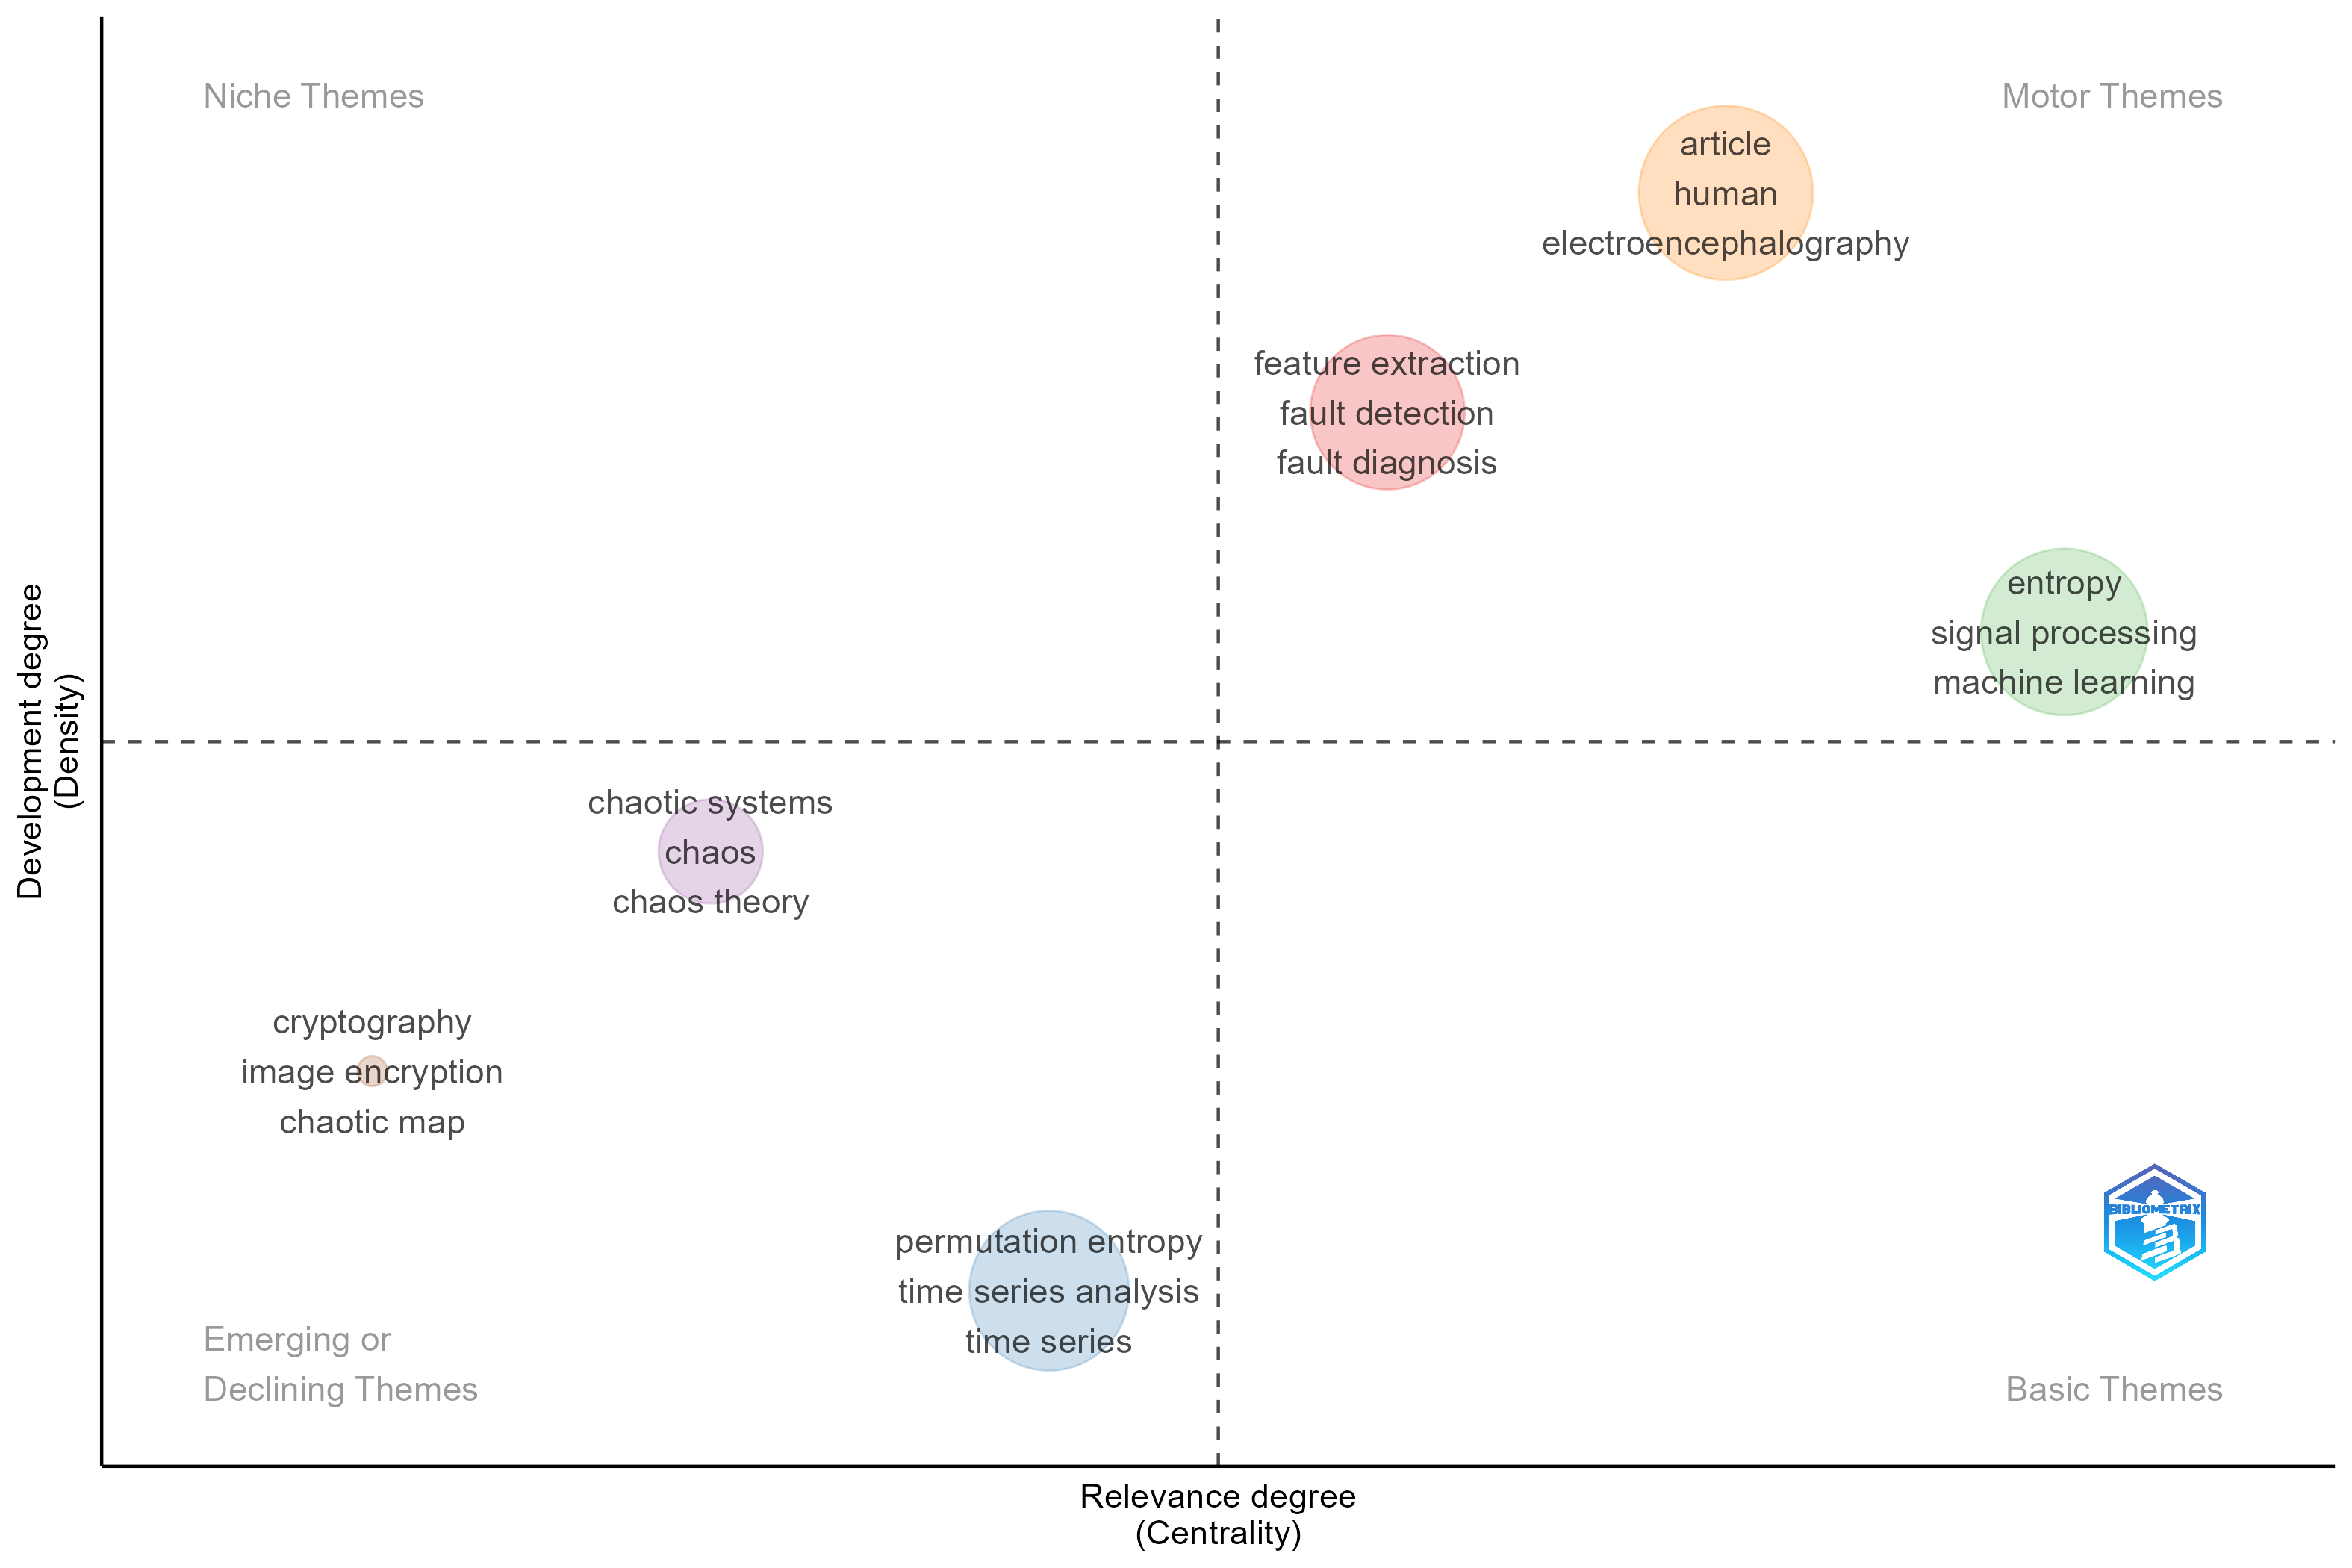
\includegraphics[width=0.9\textwidth]{ThematicMap}
	\caption{The Thematic Map generated by Biblioshiny (Bibliometrix).}
	\label{fig:ThematicMap}
\end{figure}
The map is divided into four quadrants based on two dimensions: centrality (relevance) and density (development). The quadrant representing Motor Themes includes topics such as entropy, signal processing, and machine learning, indicating well-developed and highly interconnected areas of research. Basic Themes include permutation entropy and time series analysis, which are foundational topics in the field and closely align with the focus of this thesis. Niche Themes such as chaos theory and chaotic systems represent specialized subfields, while Emerging or Declining Themes like cryptography and image encryption reflect peripheral or potentially declining research interests. This thematic analysis provides a clear framework for situating the present research within the broader academic landscape, emphasizing both its theoretical foundation and its relevance to contemporary research trends.
\begin{figure}[H]
	\centering
	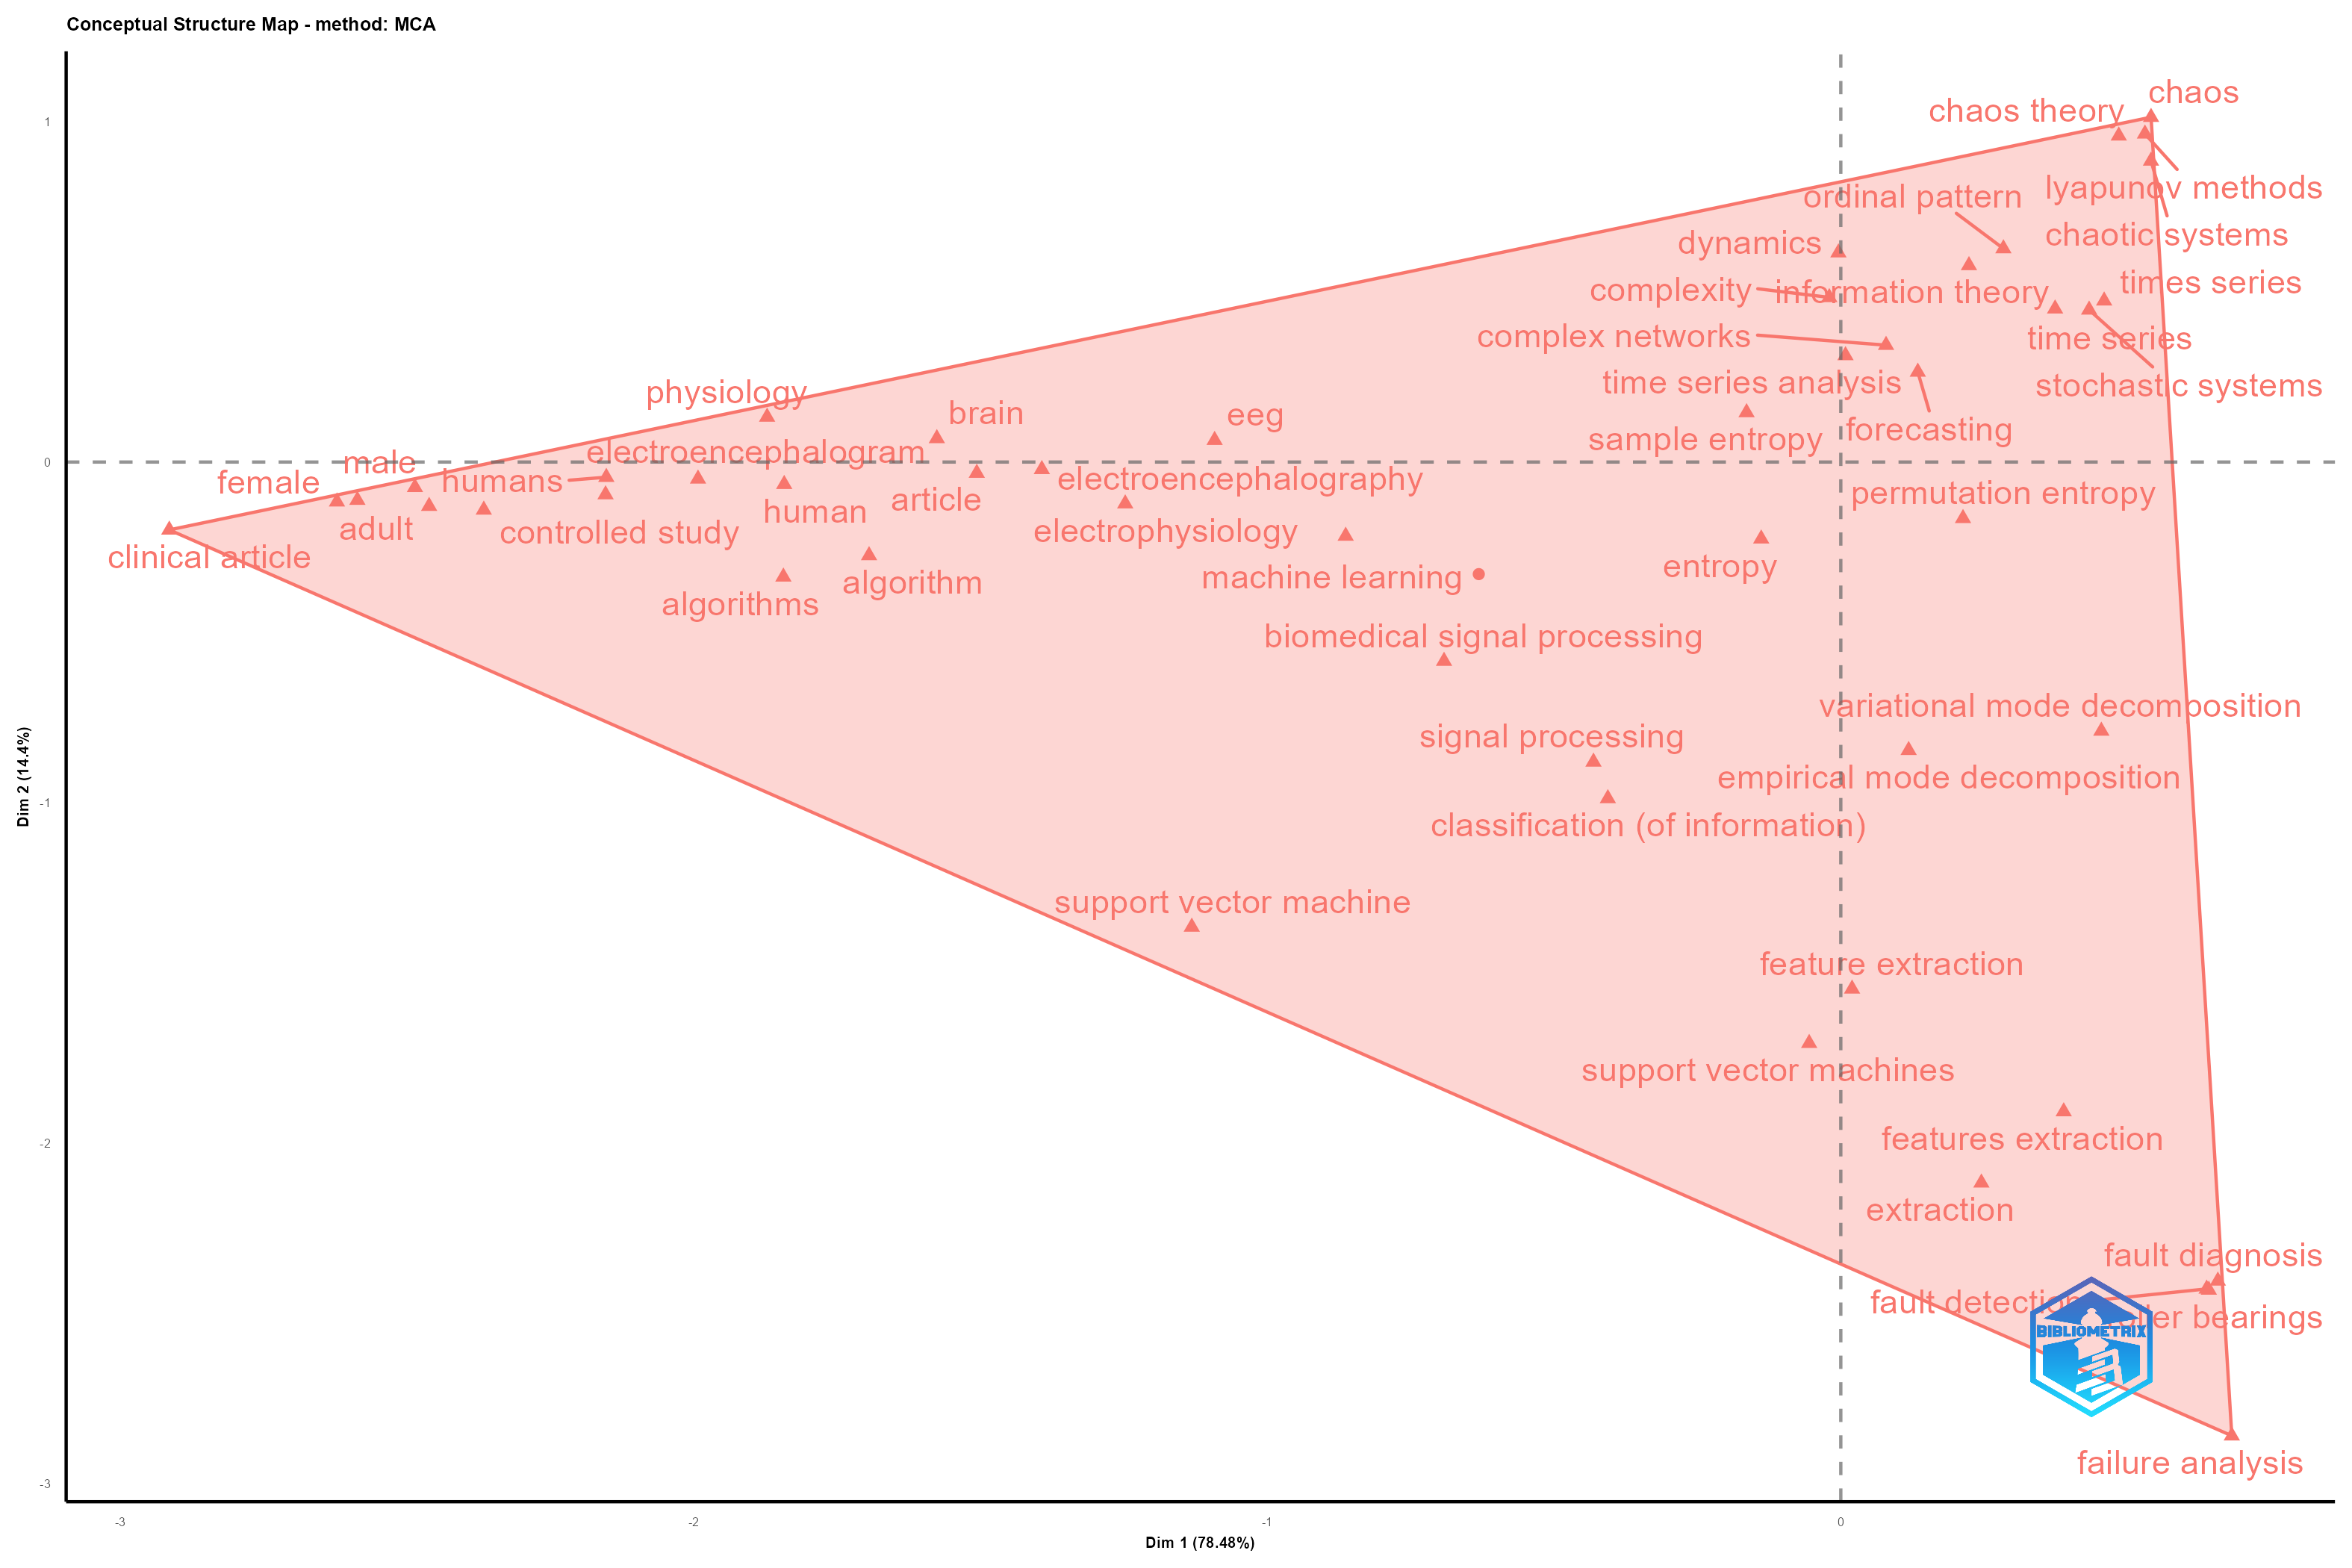
\includegraphics[width=0.9\textwidth]{FactorialMap}
	\caption{Factorial map generated by Biblioshiny (Bibliometrix).}
	\label{fig:factorialMap}
\end{figure}
The factorial map in Figure \ref{fig:factorialMap} reveals four major conceptual clusters:

The first cluster (upper right) includes theoretical concepts such as chaos theory, chaotic systems, Lyapunov methods, ordinal pattern, information theory, complex networks, and permutation entropy, forming the theoretical core of the research area.

The second cluster (lower right) includes practical applications such as feature extraction, empirical mode decomposition, variational mode decomposition, fault diagnosis, fault detection, and failure analysis, emphasizing the applied relevance of complexity-based time series analysis.

The third cluster (center) comprises terms related to biomedical signal processing and machine learning, including biomedical signal processing, EEG, support vector machine, classification, and machine learning, indicating the multidisciplinary applications of entropy measures.

A fourth, smaller cluster (left) includes clinical and physiological study keywords such as clinical article, controlled study, adult, male, female, humans, and physiology.

The factorial map thus provides further evidence of the diverse applications and theoretical development surrounding ordinal patterns and complexity measures, supporting the originality and relevance of the present research.

\section{Applications and Advances}

%%% ACF Are you going to talk about BP, or about HxC?

The Bandt-Pompe framework has since found broad applications across domains, as reviewed by Amigó et al.~\cite{amigo2023ordinal}. 
This section is divided into three subsections that analyze the applications of the Bandt and Pompe framework across various domains.

On 31 May 2025, we collected all Scopus-indexed references that cited the seminal work by Bandt and Pompe.
On that date, they were 4124.
We marked them into categories based on application fields, such as .........
 %biomedical signal processing, geophysics and hydrology, econophysics, optical systems and engineering.

\subsection{Biomedical Signal Processing}
In biomedical signal processing, it has been used to analyze EEG, ECG, and fMRI data, detecting anomalies such as epileptic seizures or sleep stage transitions. 
\begin{itemize}
	\item \textbf{EEG Analysis:} A study by Keller et al.~\cite{Keller2014} demonstrated the application of ordinal pattern based entropy measures, such as empirical permutation entropy (ePE), empirical conditional entropy (eCE), and robust empirical permutation entropy (rePE) to effectively analyze and classify EEG time series data, demonstrating their utility in detecting brain state transitions, segmenting non-stationary signals, and identifying change-points without relying on prior expert knowledge.
	
	\item \textbf{ECG Analysis:} Mansourian et al.~\cite{Mansourian2024} applied adaptive improved permutation entropy to extract fetal QRS complexes from single-channel abdominal ECG, enhancing the accuracy of fetal heart rate monitoring.
\end{itemize}

\subsection{Geophysics and Hydrology}
In the fields of geophysics and hydrology, PE has been applied to detect climatic variability and hydrological patterns.
\begin{itemize}
	\item \textbf{Climate Variability:}
	
	\item \textbf{Hydrological Patterns:}
\end{itemize}

\subsection{Econophysics, Optical Systems, and Engineering}
Permutation entropy has found applications in econophysics for market behavior analysis, in optical systems for detecting chaos, and in engineering for fault detection and diagnostics.
\begin{itemize}
	\item \textbf{Econophysics:}
	
	\item \textbf{Optical Systems:}
	
	\item \textbf{Engineering:}
\end{itemize}

\section{Methodological Extensions}
Recent developments have extended the methodology through multiscale approaches, cross-entropy comparisons for multivariate signals, and weighted ordinal patterns.

Furthermore, the use of alternative entropy measures such as Tsallis and Renyi entropy has been explored to better capture non-extensive and multifractal behavior in complex systems.

Recent developments have extended the methodology through multiscale approaches, cross-entropy comparisons for multivariate signals, and weighted ordinal patterns. These innovations aim to enhance the sensitivity of ordinal analysis across multiple temporal resolutions, account for signal interdependencies, and assign importance to certain ordinal patterns based on domain-specific knowledge.

Furthermore, the use of alternative entropy measures such as Tsallis and Rényi entropy has been explored to better capture non-extensive and multifractal behavior in complex systems, especially where the assumptions of Shannon entropy may not hold.

In addition to methodological enhancements, attention has also been given to the statistical properties of entropy and complexity estimates. One key focus is the estimation of confidence intervals for descriptors such as permutation entropy and statistical complexity. These intervals provide a quantifiable measure of uncertainty, which is crucial for distinguishing significant patterns from noise, validating comparisons between different systems, and assessing the stability of observed dynamics.

Incorporating statistical inference technique, such as asymptotic variance estimation, improves the robustness and interpretability of the results. These tools enable researchers to make reliable conclusions even in cases of short time series, thereby reinforcing the utility of ordinal methods in practical applications.

\textcolor{red}{Statistical properties!}

\section{Challenges and Future Directions}
Despite its success, several challenges remain in the application and development of the Bandt-Pompe approach. One major issue is the choice of embedding parameters (dimension and delay), which significantly affect the pattern distribution. Additionally, estimating entropy and complexity reliably in short time series remains difficult, prompting the need for improved statistical inference methods such as bootstrapping and confidence interval estimation.

Amigó et al.~\cite{amigo2023ordinal} emphasize the need for more robust inferential frameworks, better handling of multivariate and high-dimensional data, and integrating ordinal methods with machine learning for automated pattern recognition. As ordinal symbolic analysis continues to evolve, it holds promise for deeper insights into both theoretical dynamics and real-world systems.

As a final conclusion related to this literature review, the Bandt-Pompe method has become a foundational tool in time series analysis, offering a robust and intuitive approach to understanding complex dynamics. Through the use of ordinal patterns and entropy-based descriptors, researchers can extract meaningful information from noisy, nonlinear, and non-stationary data. While challenges remain, ongoing theoretical advances and applications across disciplines ensure the continued relevance and growth of this methodology.





